% !TEX TS-program = xelatex
% !TEX encoding = UTF-8

% This is a simple template for a XeLaTeX document using the "article" class,
% with the fontspec package to easily select fonts.

\documentclass[11pt]{article} % use larger type; default would be 10pt

\usepackage{fontspec} % Font selection for XeLaTeX; see fontspec.pdf for documentation
\defaultfontfeatures{Mapping=tex-text} % to support TeX conventions like ``---''
\usepackage{xunicode} % Unicode support for LaTeX character names (accents, European chars, etc)
\usepackage{xltxtra} % Extra customizations for XeLaTeX

%\setmainfont{Charis SIL} % set the main body font (\textrm), assumes Charis SIL is installed
%\setsansfont{Deja Vu Sans}
%\setmonofont{Deja Vu Mono}
\setmainfont[Mapping=tex-text]{TeX Gyre Pagella}
%\setsansfont[Mapping=tex-text]{Helvetica}

% other LaTeX packages.....
\usepackage{geometry} % See geometry.pdf to learn the layout options. There are lots.
\geometry{a4paper} % or letterpaper (US) or a5paper or....
%\usepackage[parfill]{parskip} % Activate to begin paragraphs with an empty line rather than an indent

\usepackage{graphicx} % support the \includegraphics command and options

\title{Colibrys SF3000 Signal-to-Noise Ratio Measurement of KM Tower (Ambient Vibration)\\DAQ : ANYLOGGER 4CH}
\author{Korea Maintenance Co., LTD.}
%\date{} % Activate to display a given date or no date (if empty),
         % otherwise the current date is printed 

\begin{document}
\maketitle
\clearpage
\section{KM Tower X-dir Measurement}
Max Level = -20.0dB/Hz\\
Noise Level = -137.3dB/Hz\\
\textbf{SNR=117.3dB}
\begin{figure}[!hbpt]
\centering
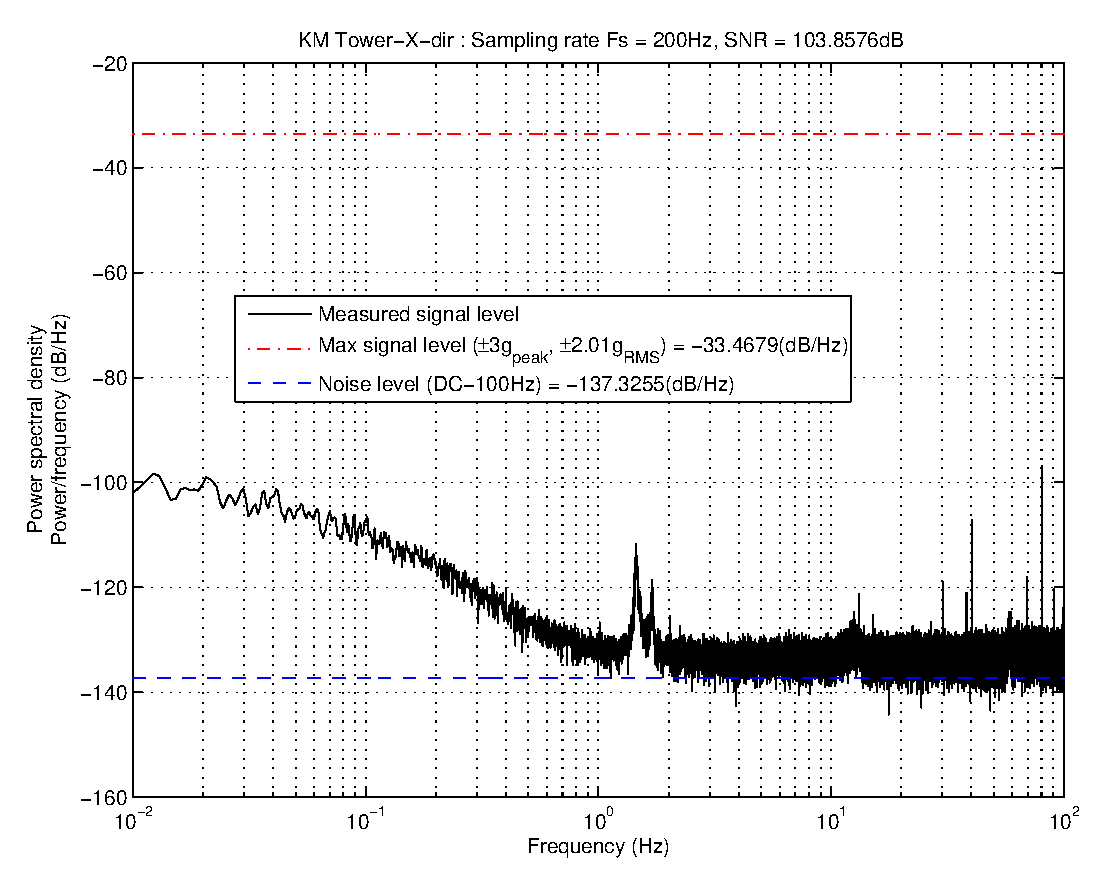
\includegraphics[keepaspectratio=true,width=1\linewidth]{figs/KMTower-X-dir.eps}
\caption{Power spectral density of KM Tower X-direction}
\label{fig:psd1}
\end{figure}

\clearpage
\section{KM Tower Y-dir Measurement}
Max Level = -20.0dB/Hz\\
Noise Level = -135.5dB/Hz\\
\textbf{SNR=115.5dB}
\begin{figure}[!hbpt]
\centering
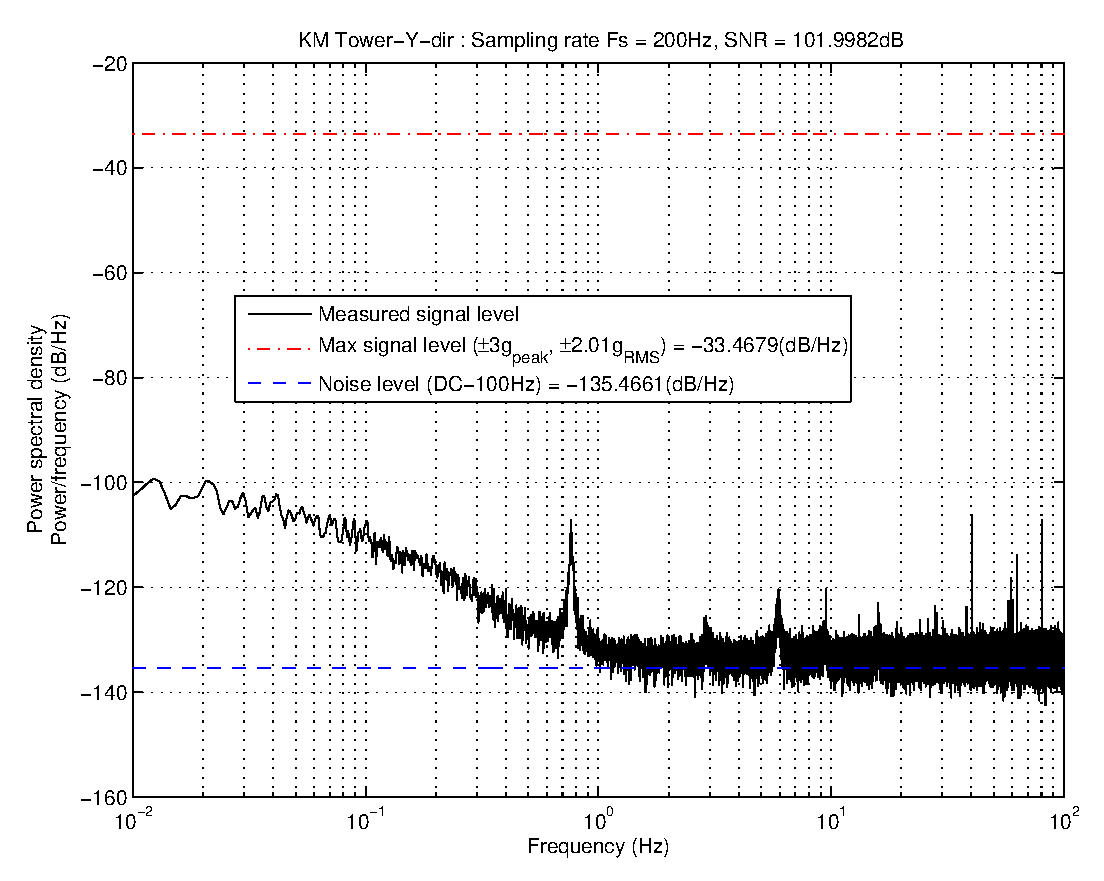
\includegraphics[keepaspectratio=true,width=1\linewidth]{figs/KMTower-Y-dir.eps}
\caption{Power spectral density of KM Tower Y-direction}
\label{fig:psd2}
\end{figure}

\clearpage
\section{KM Tower Z-dir Measurement}
Max Level = -20.0dB/Hz\\
Noise Level = -134.3dB/Hz\\
\textbf{SNR=114.4dB}
\begin{figure}[!hbpt]
\centering
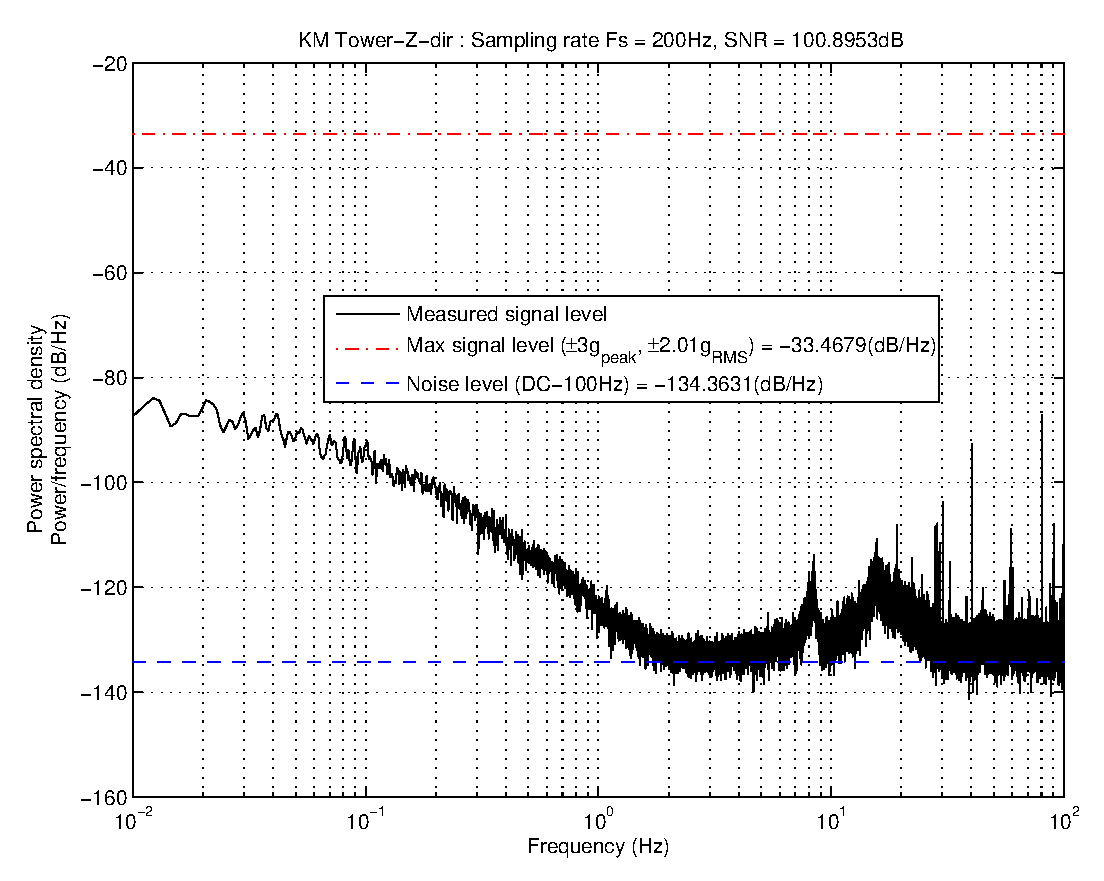
\includegraphics[keepaspectratio=true,width=1\linewidth]{figs/KMTower-Z-dir.eps}
\caption{Power spectral density of KM Tower Z-direction}
\label{fig:psd3}
\end{figure}
%\section{}

%\subsection{}



\end{document}
